%!TEX root=main.tex
\section[Aufbau des Auges\hfill Aufbau der Materie]{Aufbau des Auges\\{\normalsize Aufbau der Materie}}
\label{sec:auge}
% Das visuelle System dient zur Verarbeitung visueller Information und umfasst Auge, Sehnerv und Teile des Gehirns.

% \subsection{Das Auge}
Das Auge ähnelt in seiner Funktion einer Kamera. Die Linse (das Objektiv) sammelt Lichtstrahlen und projiziert diese als auf dem Kopf stehendes gespiegeltes Bild auf die Netzhaut (den Film). Da der Abstand zwischen Linse und Netzhaut (die Bildweite) unveränderlich ist, muss die Brechkraft (Brennweite) der Augenlinse angepasst werden. Diese Anpassung nennt man \textit{Akkommodation}.

\begin{figure}
	\centering
	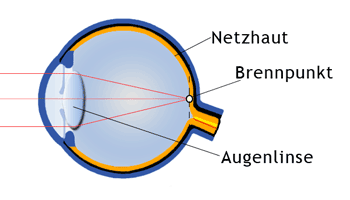
\includegraphics[width=4.5cm]{images/auge.png}
	\caption{Auge \cite{abadi:fehlsichtigkeit}}
\end{figure}

Die Projektion wird von lichtempfindlichen Sehzellen, den \textit{Photorezeptoren} in elektrische Nervenimpulse umgewandelt und über den Sehnerv an das Gehirn weitergeleitet.

\begin{figure}
	\centering
	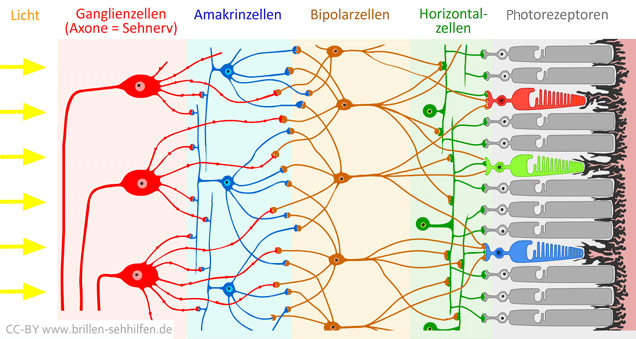
\includegraphics[width=10cm]{images/netzhaut.png}
	\caption{Sehzellen der Netzhaut \cite{bs:auge}}
\end{figure}

Die Photorezeptoren werden 